\documentclass{beamer}
\usetheme{Madrid}

\usepackage{amsmath, amssymb, amsthm}
\usepackage{graphicx}
\usepackage{gensymb}
\usepackage[utf8]{inputenc}
\usepackage{hyperref}
\usepackage{tikz}

\bibliographystyle{IEEEtran}
\vspace{3cm}

\title{1.2.12}
\author{AI25BTECH11006 - Nikhila}
\date{27-08-25}

\begin{document}

\frame{\titlepage}

% Question frame
\begin{frame}
\frametitle{Question}
If the points \textbf{A}(6,1),\textbf{B}(8,2),\textbf{C}(9,4) and \textbf{D}(p,3) are the vertices of a parallelogram,taken in order. find the value of p .
\\\end{frame}




% Solution steps
\begin{frame}
\frametitle{Solution}
The given the points $\textbf{A}\begin{pmatrix}6 \\ 1 \end{pmatrix} , \textbf{B}\begin{pmatrix}8 \\ 2\end{pmatrix} , \textbf{C}\begin{pmatrix}9 \\ 4\end{pmatrix}$ and $\textbf{D}\begin{pmatrix}p \\ 3\end{pmatrix}$\\
\vspace{1em}
 If ABCD be a parallelogram with AB $||$ CD ,
\begin{align*}
\textbf{$\textbf{B}-\textbf{A} = \textbf{C}-\textbf{D}$}
\end{align*}
 \end{frame}



\begin{frame}
\frametitle{Solution}
The vector components are:
\begin{align}
   \textbf{B} - \textbf{A} =\begin{pmatrix}8 \\ 2\end{pmatrix} - \begin{pmatrix}6 \\ 1\end{pmatrix} = \begin{pmatrix}2 \\ 1\end{pmatrix}\\
   \textbf{C}- \textbf{D}=\begin{pmatrix}9 \\ 4\end{pmatrix} - \begin{pmatrix}p \\ 3\end{pmatrix} = \begin{pmatrix}9-p \\ 1\end{pmatrix}
\end{align}
By comparing 
\begin{align}
    9-p = 2
\end{align}
We get 
\begin{align}
    p = 7
\end{align}

\end{frame}

% Graphical representation
\begin{frame}
\frametitle{Graphical Representation}
Hence the coordinates of \textbf{D} are (7 , 3)
\begin{center}
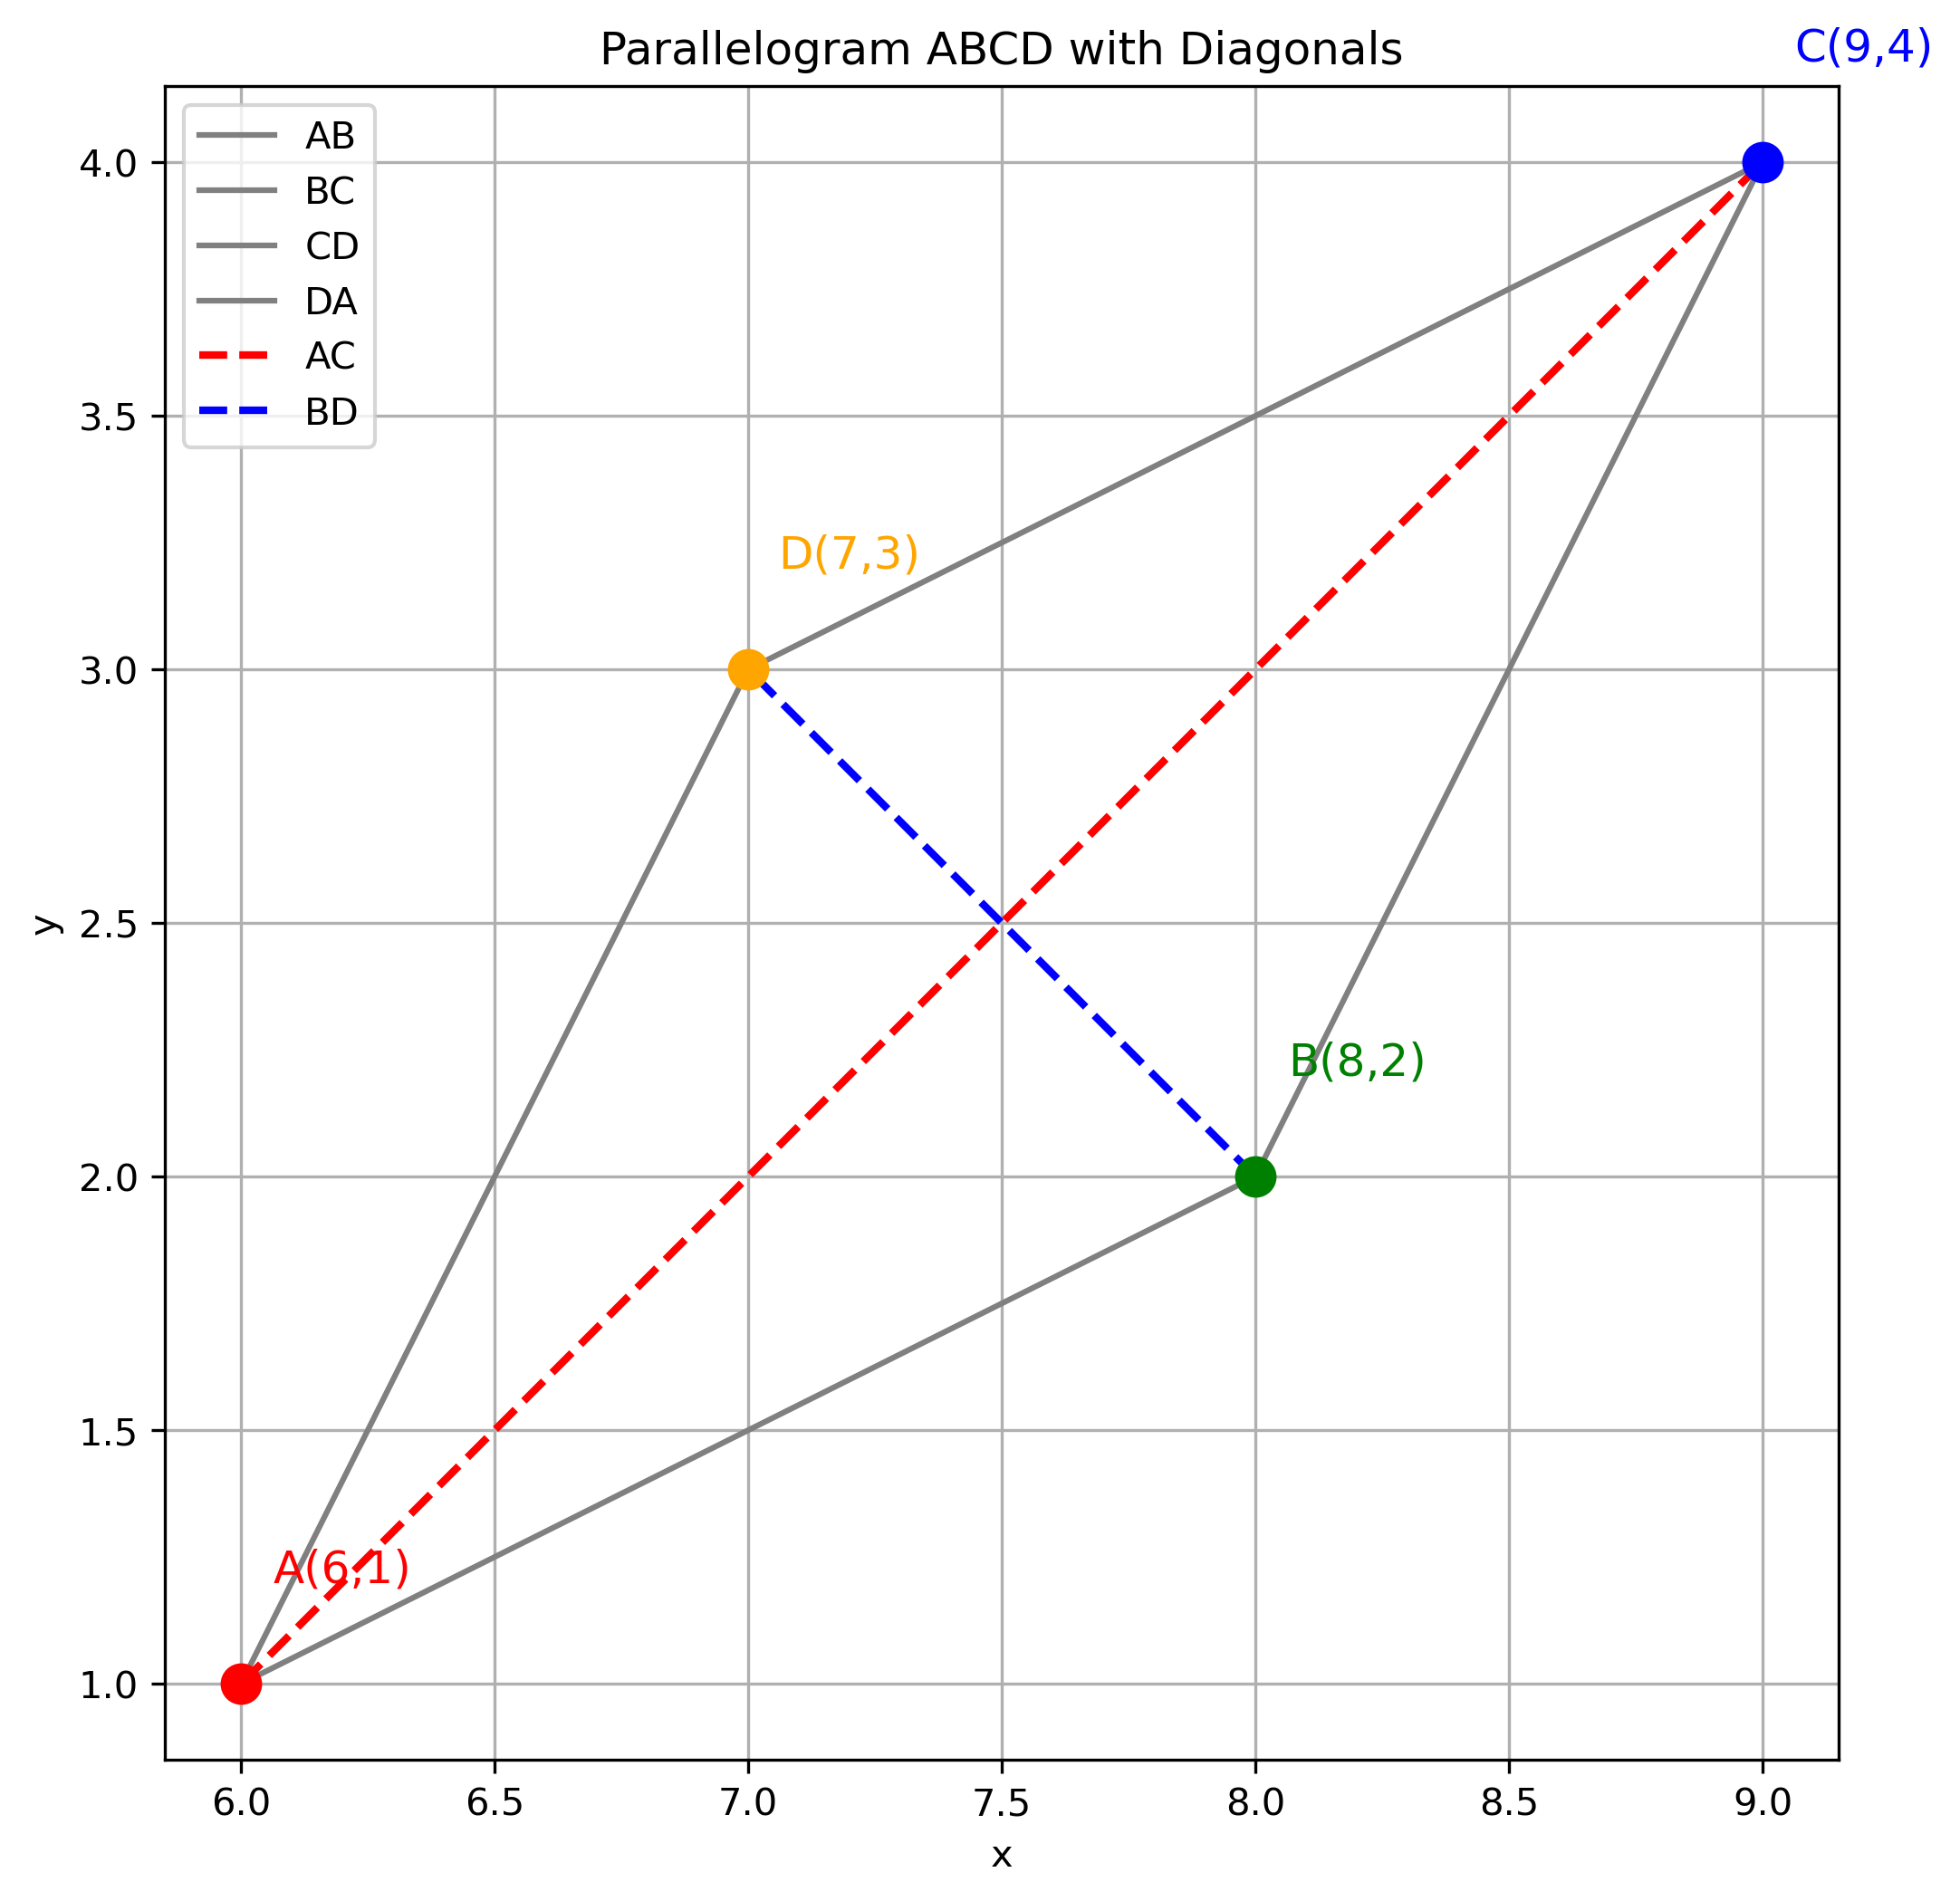
\includegraphics[width=0.6\linewidth]{fig1.png}
\end{center}
\end{frame}

\end{document}
